\documentclass[a4paper,11pt]{report}

\usepackage{amsmath,amssymb}
\usepackage{fullpage}
\usepackage{graphicx}

\usepackage{bussproofs}
\usepackage{mathpartir}
\usepackage{prooftrees}
\usepackage{color}

\usepackage{tikz}
\usetikzlibrary{automata,positioning}

\newcommand*\circled[1]{\tikz[baseline=(char.base)]{
            \node[shape=circle,draw,inner sep=2pt] (char) {#1};}}

\makeatletter
\pgfmathdeclarefunction{alpha}{1}{%
  \pgfmathint@{#1}%
  \edef\pgfmathresult{\pgffor@alpha{\pgfmathresult}}%
}

\newcommand*{\until}{U}
\newcommand*{\disj}{\ ,\ }
\newcommand*{\A}{\square}  % Always
\newcommand*{\D}{\diamondsuit} % eventually

\newcommand*{\Pq}{(\top,\bot)}
\newcommand*{\pQ}{(\bot,\top)}
\newcommand*{\PQ}{(\top,\top)}
\newcommand*{\pq}{(\bot,\bot)}

% tikz
\usepackage{tikz}
\usetikzlibrary{snakes}

\author{Sylvain Julmy}
\date{\today}

\setlength{\parindent}{0pt}
\setlength{\parskip}{2.5pt}

\begin{document}

\begin{center}
\Large{
    Automata on Infinite Structure\\
    Fall 2018
  }
  
  \noindent\makebox[\linewidth]{\rule{\linewidth}{0.4pt}}
  Exercice Sheet 2

  \vspace*{1.4cm}

  Author : Sylvain Julmy
  \noindent\makebox[\linewidth]{\rule{\linewidth}{0.4pt}}

  \begin{flushleft}
    Professor : Ultes-Nitsche Ulrich
    
    Assistant : Stammet Christophe
  \end{flushleft}

  \noindent\makebox[\linewidth]{\rule{\textwidth}{1pt}}
\end{center}

\section*{Exercice 1}

\[
  L_\omega(A_1) = ((a|c)^*(b((a|c)|(b(a|c))) ))^\omega
\]

\[
A_2 =
\]

\begin{center}
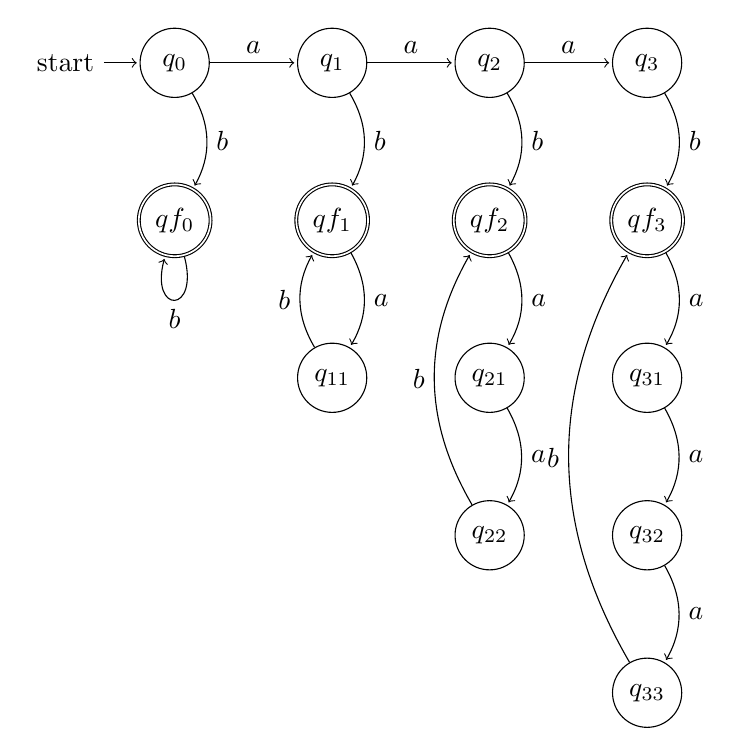
\begin{tikzpicture}[shorten >=1pt,node distance=2cm,on grid,auto]
  \node[state,initial] (q0) {$q_0$};
  \node[state] (q1) [right = of q0] {$q_1$};
  \node[state] (q2) [right = of q1] {$q_2$};
  \node[state] (q3) [right = of q2] {$q_3$};
  
  \node[state,accepting] (qf0) [below = of q0] {$qf_0$};
  \node[state,accepting] (qf1) [right = of qf0] {$qf_1$};
  \node[state,accepting] (qf2) [right = of qf1] {$qf_2$};
  \node[state,accepting] (qf3) [right = of qf2] {$qf_3$};
  
  \node[state] (q11) [below = of qf1] {$q_{11}$};
  \node[state] (q21) [below = of qf2] {$q_{21}$};
  \node[state] (q31) [below = of qf3] {$q_{31}$};
  
  \node[state] (q22) [below = of q21] {$q_{22}$};
  \node[state] (q32) [below = of q31] {$q_{32}$};
  
  \node[state] (q33) [below = of q32] {$q_{33}$};
  
  \path[->]
  (q0)
  edge [] node [] {$a$} (q1)
  edge [bend left] node [] {$b$} (qf0)
  (qf0)
  edge [loop below] node [] {$b$} ()
  (qf1)
  edge [bend left] node [] {$a$} (q11)
  (qf2)
  edge [bend left] node [] {$a$} (q21)
  (qf3)
  edge [bend left] node [] {$a$} (q31)
  (q21)
  edge [bend left] node [] {$a$} (q22)
  (q31)
  edge [bend left] node [] {$a$} (q32)
  (q32)
  edge [bend left] node [] {$a$} (q33)
  (q1)
  edge [] node [] {$a$} (q2)
  edge [bend left] node [] {$b$} (qf1)
  (q2)
  edge [] node [] {$a$} (q3)
  edge [bend left] node [] {$b$} (qf2)
  (q3)
  edge [bend left] node [] {$b$} (qf3)
  (q11)
  edge [bend left] node [] {$b$} (qf1)
  (q22)
  edge [bend left] node [] {$b$} (qf2)
  (q33)
  edge [bend left] node [] {$b$} (qf3)
  ;
\end{tikzpicture}
\end{center}

To compute $|Q|$ and $|F|$ from $k$, we see that each time we add $1$ to $k$, we
have an additional column $qk_i = (q_i,qf_i,q_{i1},\dots,q_{ii})$ where $i$ is
the value of $k$. Each such column has one more element than the previous so we
can compute $|Q| = 2 + 3 + 4 + 5 + \dots + (k+2) = \frac{(k+2)(k+3)}{2} - 1$.
Then each time we increment $k$, we need one more final state, so $|F| =
\underbrace{1 + 1 + 1 + \dots}_{k+1}$.

\section*{Exercice 2}

\subsection*{a)}

\[
A_{1 \cup 2} = 
\]


\begin{center}
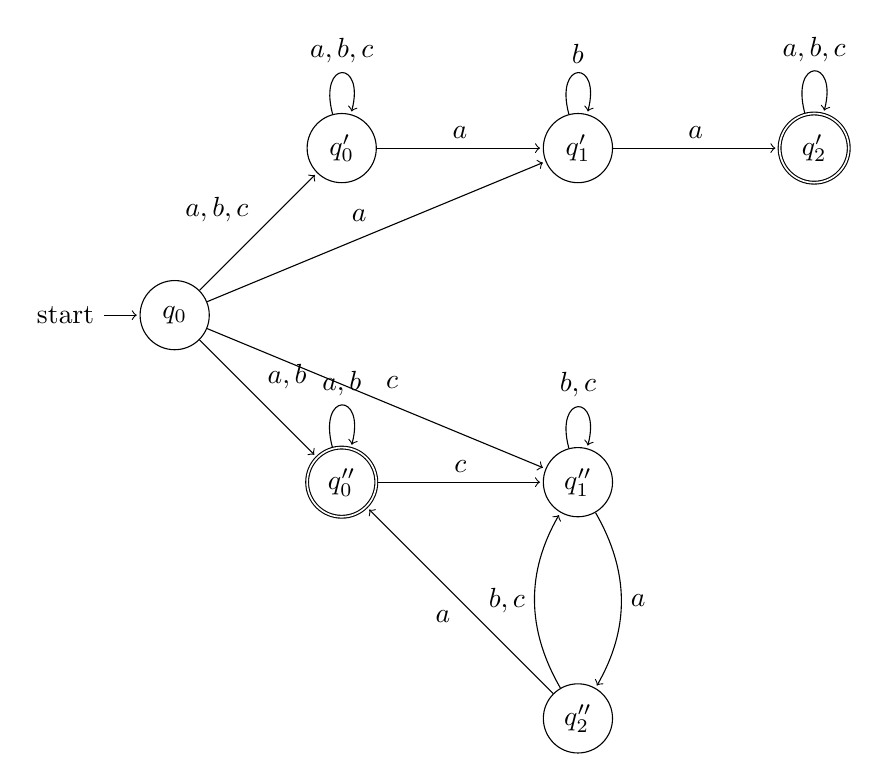
\begin{tikzpicture}[shorten >=1pt,node distance=3cm,on grid,auto]
  \node[state,initial] (q0) {$q_0$};
  \node[state] (q0') [above right = of q0] {$q_0'$};
  \node[state] (q1') [right = of q0'] {$q_1'$};
  \node[state,accepting] (q2') [right = of q1'] {$q_2'$};
  \node[state,accepting] (q0'') [below right = of q0] {$q_0''$};
  \node[state] (q1'') [right = of q0''] {$q_1''$};
  \node[state] (q2'') [below = of q1''] {$q_2''$};
  \path[->]
  (q0)
  edge [] node [] {$a,b,c$} (q0')
  edge [] node [] {$a$} (q1')
  edge [] node [] {$a,b$} (q0'')
  edge [] node [] {$c$} (q1'')
  (q0')
  edge [loop above] node [] {$a,b,c$} ()
  edge [] node [] {$a$} (q1')
  (q1')
  edge [loop above] node [] {$b$} ()
  edge [] node [] {$a$} (q2')
  (q2')
  edge [loop above] node [] {$a,b,c$} ()
  (q0'')
  edge [loop above] node [] {$a,b$} ()
  edge [] node [] {$c$} (q1'')
  (q1'')
  edge [loop above] node [] {$b,c$} ()
  edge [bend left] node [] {$a$} (q2'')
  (q2'')
  edge [] node [] {$a$} (q0'')
  edge [bend left] node [] {$b,c$} (q1'')
  ;
\end{tikzpicture}
\end{center}

\subsection*{b)}

\[
A_{1 \cap 2} = 
\]


\begin{center}
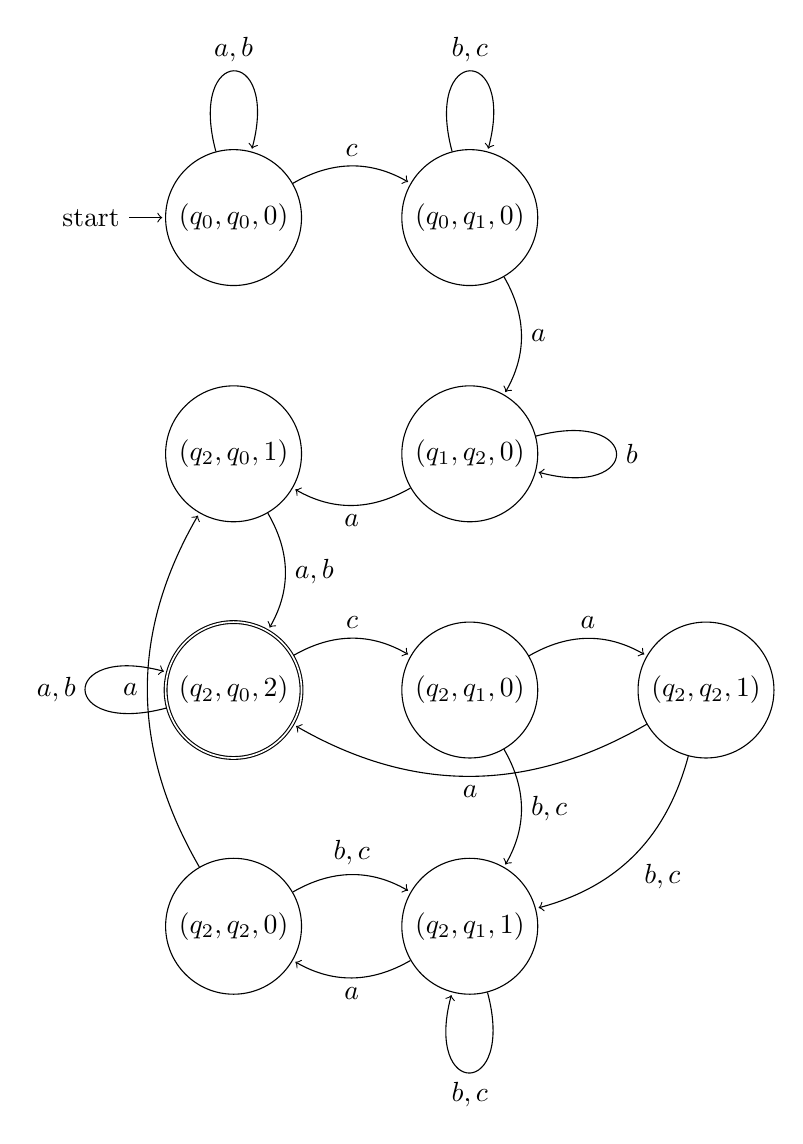
\begin{tikzpicture}[shorten >=1pt,node distance=3cm,on grid,auto]
  \node[state,initial] (q0q00) {$(q_0,q_0,0)$};
  
  \node[state] (q0q10) [right = of q0q00] {$(q_0,q_1,0)$};
  \node[state] (q2q01) [below = of q0q00] {$(q_2,q_0,1)$};
  \node[state] (q1q20) [right = of q2q01] {$(q_1,q_2,0)$};
  \node[state,accepting] (q2q02) [below = of q2q01] {$(q_2,q_0,2)$};
  \node[state] (q2q10) [right = of q2q02] {$(q_2,q_1,0)$};
  \node[state] (q2q20) [below = of q2q02] {$(q_2,q_2,0)$};
  \node[state] (q2q11) [right = of q2q20] {$(q_2,q_1,1)$};
  \node[state] (q2q21) [right = of q2q10] {$(q_2,q_2,1)$};
  
  \path[->]
  (q0q00)
  edge [loop above] node [] {$a,b$} ()
  edge [bend left] node [] {$c$} (q0q10)
  (q0q10)
  edge [loop above] node [] {$b,c$} ()
  edge [bend left] node [] {$a$} (q1q20)
  (q1q20)
  edge [loop right] node [] {$b$} ()
  edge [bend left] node [] {$a$} (q2q01)
  (q2q01)
  edge [bend left] node [] {$a,b$} (q2q02)
  (q2q02)
  edge [loop left] node [] {$a,b$} ()
  edge [bend left] node [] {$c$} (q2q10)
  (q2q10)
  edge [bend left] node [] {$b,c$} (q2q11)
  edge [bend left] node [] {$a$} (q2q21)
  (q2q11)
  edge [loop below] node [] {$b,c$} ()
  edge [bend left] node [] {$a$} (q2q20)
  (q2q20)
  edge [bend left] node [] {$a$} (q2q01)
  edge [bend left] node [] {$b,c$} (q2q11)
  (q2q21)
  edge [bend left] node [] {$a$} (q2q02)
  edge [bend left] node [] {$b,c$} (q2q11)
  ;
\end{tikzpicture}
\end{center}


\section*{Exercice 3}

\subsection*{a)} Recognize any word that contains a finite sequence of $b$ in
between of $2$ $a$ : $\dots abbbbbb \dots bbba \dots$. Regular expression :
$(a|b|c)^*ab^*a(a|b|c)^\omega$.

\subsection*{b)}

Recognize any word that end by an infite sequence of $ab$, an infite sequence of
$ac$ or an infite sequence of $b$. Regular expression : $(a|b|c)^*
((ab)^\omega|(ac)^\omega|b^\omega)$.

\end{document}